
\subsection{Take home messages for Week 1}
\hlr{Basic concepts for Group Theory}

群的定义有两个推论,并不是显然的
\begin{itemize}
  \item 单位元是唯一的,所有$ ka = a $那么$ k $必然是单位元
  \item 逆元是唯一的,$ ab = e $,不可能有两个逆元
\end{itemize}
对于有限群来说,可约表示意味着有不变子空间。也就是存在一个投影算符投影到不变子空间上面。这个是最本质的定义!!$ P D P = D P $。

对于Completely Reducible的定义是:存在一组不等价不可约表示的直和构成!

Transformation Group是对于物理进行定义的。一些特殊的坐标变换,我们物理上认为是Symmetry Transformation。这些变换构成了群结构。并且量子力学公理告诉我们量子态按照这些群在Hilbert空间上的表示进行变换。

比如:空间反演变换构成$ \mathbb{Z}_2 $群,所以我们如果空间反演和H对易,则Hamiltonian的本征态按照$ \mathbb{Z}_2 $群的表示进行变换。也就是有的不变(态在trivial表示空间)有的$ \times -1 $(态在non-trivial表示空间)。

\hlr{
There are two Thm for finite group representations:
}
\thm{
  所有有限群的表示都等价于一个Unitary的表示!
}
\thm{所有有限群的表示都是完全可约的!!就是由一堆不等价不可约表示直和构成!!}
\thm{
  Abelian group的所有不等价不可约表示都是1维的
}

\hlr{All kinds of concept for subgroup}

\defi{Invriant Subgroup

  A subgroup $ H \subset G $ that satisfy: $ \forall g \in G, g^{-1}Hg = H $. From this we can define the quotient group (factor group) $ G/H $. Which we can see that all right coset (gH) of invariant subgroup froms a group.
}
\imp{factor group表示}{
我们注意,如果一个表示作用在一个invariant subgroup上面,对应的线性算子是一模一样的。那么这个表示同时也是factor group的一个表示!!

同样的对于factor group的表示也是原来group的一个表示!!
}
\defi{Conjugation class

  A set of group elements $ S $ that satisfy: $ \forall g \in G, g^{-1}Sg = S $.
}
\hlr{Shur's Lemma and its applications in QM}

\imp{Shur's Lemma}{
\begin{itemize}
  \item 对于两个不等价不可约表示$ D_1,D_2 $,如果存在一个线性算子$ A $使得$ AD_1(g) = D_2(g)A $那么$ A = 0 $
  \item 对于一个不可约表示$ D $,如果存在一个线性算子$ A $使得$ AD(g) = D(g)A $那么$ A = \lambda I $
\end{itemize}
}


\imp{Shur引理的量子力学结论}{
  根据shur Lemma我们知道,如果一个算符和所有不等价不可约表示对易那么这个算符必然正比与单位矩阵。

  量子力学里面存在Scalar Observabes,他们的定义就是,对于一个坐标变换前后算符形式完全不变:
  \begin{equation}
    T' = D(g) T D(g)^{\dagger} = T \quad \forall g \in G
    \label{eq:scalarobs}
  \end{equation}
  那么对于这样的算符来说,显然有一个不等价不可约表示和其对易,那么在这样的不等价不可约表示空间上面,$ T $必然正比于单位矩阵!!用数学的语言表达就是这样的算符在不等价不可约表示空间上面是:
  \begin{equation}
    \langle a,j,x|O|b,k,y\rangle=f_a(x,y)\delta_{ab}\delta_{jk}
    \label{eq:scalartrans}
  \end{equation}

  scalar observables 是Tensor observables的一个特例,所以这个也是wiger-Eckart theorem的一个特例!!

  \textbf{Note that我们对于同样的表示,使用一模一样的基$ \ket{b,k} $ 所以也就只有一个指标$ x,y $来区分不同的表示}

}
\hlr{Orthogonality of representations}
\thm{不等价不可约表示的正交性

一个有限群的全部不等价不可约Unitary表示,构成了群元素作为lebal的一组正交归一完备基!其归一化是:
\begin{equation}
  \sum_{g\in G}\frac{n_a}{N}[D_a(g)]_{jk}^*[D_b(g)]_{\ell m}=\delta_{ab}\delta_{j\ell}\delta_{km}
  \label{eq:shurorthonormal}
\end{equation}
需要注意哪两个指标是互相正交的。
}
\textbf{一个显然的重要推论:}对于一个有限群我们有【群的order等于所有不等价不可约Unitary表示的维度平方和】
\begin{equation}
  N = \sum_a n_a^2
  \label{eq:burnthm}
\end{equation}
\thm{群函数的基

  我们现在意识到了,正交性的存在意味着所有不等价不可约表示的分量构成了群函数的完备基!!也就是对于所有满足:
  \begin{equation}
    F(g) = \sum_a \sum_{jk} f_a^{jk} [D_a(g)]_{jk}
    \label{eq:groupfunction}
  \end{equation}
}

\hlr{Character of representation}
\imp{Character}{
  特征标是对于【某一个表示】的【某一个群元素】定义的:
  \begin{equation}
    \chi_D(g)\equiv\operatorname{Tr}D(g)=\sum_i[D(g)]_{ii}
    \label{eq:character}
  \end{equation}
  特征标的一个重要性质是:对于相似变换不变,也就是对于所有等价的表示是不变的。
  \begin{enumerate}
    \item character 根据表示的正交性有正交性:
      \begin{equation}
        \frac{1}{N}\sum_{g\in G}\chi_{D_a}(g)^*\chi_{D_b}(g)=\delta_{ab}
        \label{eq:cahracterorthogonality}
      \end{equation}
      注意,虽然character是类函数,但是这里是对于所有群元素进行求和,如果是对于类求和还需要乘以类的大小.
\begin{equation}
  \sum_a\chi_{D_a}\left(g_\alpha\right)^*\chi_{D_a}\left(g_\beta\right)=\frac{N}{k_\alpha}\delta_{\alpha\beta}
  \label{eq:columnorthonality}
\end{equation}
这两种正交性可以统一的用一种写法写出来:$ V_{\alpha a}=\sqrt{\frac{k_\alpha}{N}}\chi_{D_a}(g_\alpha) $结论就是$ V V^\dagger = V^\dagger V = 0 $而这个V矩阵是一个Unitary矩阵也就是character table(当然,需要乘上一些系数)!

    \item character 是所有关于g的conjugation invariant function的完备基!! 也就是对于所有满足:$ F(g)  = F(g_1^{-1}g g_1)$ 的函数。其实就是类函数的一组完备基,因为\textbf{同一个conjugation class}的character是一样的。所以这样的conjugation invariant function其实是关于conjugation class的函数!!
    \item 不等价不可约表示的数量 = conjugation class的数量
    \item 对于一个reducable rep来说,其包含某个irr rep的数量可以通过character计算出来:
      \begin{equation}
        m_a^D = \frac{1}{N}\sum_{g\in G}\chi_D(g)^*\chi_{D_a}(g)
        \label{eq:reducablenumber}
      \end{equation}
      这个公式是非常重要的!!!
      \item 表示的张量积的character是各个表示character的乘积:
        \begin{equation}
          \chi_{D_1\otimes D_2}(g) = \chi_{D_1}(g)\chi_{D_2}(g)
          \label{eq:tensorproductcharacter}
        \end{equation}
  \end{enumerate}
}

\hlr{给定群如何得到character表,以及如何利用character表进行约化?}

\textbf{Step 1: } 列出群元素,乘法关系,最终给出所有的conjugation class。其中可以利用burnside定理帮助确定有几个conjugation class。

\textbf{Step 2: }根据burnside定理确定有几个不等价不可约表示。并且根据$ \sum_a n_a^2 = N $确定每个表示的维度。

\textbf{Step 3: }可以根据不变子群的性质,通过研究factor group来确定一些低维表示。并给出表示的character。

\textbf{Step 4: }利用正交性确定剩下的表示的character。得到character表!

\imp{character构建可约表示的不等价不可约表示子空间的基}{
  我们通过不等价不可约表示的character构造一个投影算符,这个投影算符作用在可约表示的基啥昂面的时候就得到了这个不等价不可约表示的子空间的基,在可约表示的空间上的样子!
\begin{equation}
  P_a=\frac{n_a}{N}\sum_{g\in G}\chi_{D_a}(g)^*D(g)
  \label{eq:projectortoirr}
\end{equation}

}

\hlr{QM application of group representation theory}
\thm{如果一个对称变换对于Hermite Operator H是对易的。那么
\begin{itemize}
  \item H的本征态的同Eigen Value的本征态空间可以约化成这个对称性变换不等价不可约表示的直和。
  \item 如果一个不等价不可约表示只出现一次,那么这个表示空间的所有向量都是H的本征态,并且本征值完全相同。
\end{itemize}
}



\subsection{Explanations and Questions for Week 1}

\textbf{Question 1: What is the relation between Z3 group 3dim representation and the SO(3) group 3dim representation?} 

We can see that the Z3 group 3dim rep is a subset of SO(3) and it represent the rotation of 120 degree along the axis of (1,1,1) direction. 

\begin{equation}
  \begin{gathered}D(e)=\begin{pmatrix}1&0&0\\0&1&0\\0&0&1\end{pmatrix},\quad D(a)=\begin{pmatrix}0&0&1\\1&0&0\\0&1&0\end{pmatrix}\\D(b)=\begin{pmatrix}0&1&0\\0&0&1\\1&0&0\end{pmatrix}\end{gathered}
  \label{eq:z3rep3}
\end{equation}


\tip{How to get regular representation}{
  \textbf{The first approach :} we assign vecotrs for the group element that are orthogonal to each other. This is basis invariant so why not choose a basis that has (1,0,0),(0,1,0),(0,0,1) as vectors for a 3 order group.

  However, we can also perform basis invariant calculation as:
  \begin{equation}
\begin{aligned}
|e_1\rangle &= |e\rangle ,\quad |e_2\rangle = |a\rangle ,\quad |e_3\rangle = |b\rangle \\ 
[D(g)]_{ij} &= \langle e_i|D(g)|e_j\rangle 
\end{aligned}
\label{eq:basisinvZ3}
\end{equation}

}

\imp{本书之中重大问题}{
我需要强调,本书之中混淆了operator以及matrix的区别。

矩阵是数值捏。数值可以因为主动变换【operator进行变换】或者被动变化【基进行变换】两种思考进行变换呀呀呀!!
}

\tip{线性空间算子}{
  我们需要注意一点,就是区分矩阵和线性空间的算子。

  线性算子是两个线性空间之间的映射。只有确定一个基才能够写作一个矩阵的形式捏!!矩阵更像是某一个基下面的线性算子的表示。

\bigskip

  但是两者还是有很深刻的联系的。比如,如果我们选择了一个基,(1,0,0),(0,1,0),(0,0,1)那么,其实线性空间的算子可以构建出这样基作为regular表示的元素对应的基的矩阵也就是:
\begin{equation}
[D(g)]_{ij} = \langle e_i|D(g)|e_j\rangle 
  \label{eq:operatortomatrix}
\end{equation}

\textbf{一句话概括:他们的区别就是像是张量和张量的分量的区别。operator是几何物体;matrix是具体的数字是代数}

  这就牵扯出了一个问题,就像张量一样,如果我们想对比一个抽象不变量的具体情况我们需要fix一些东西才能比较不同。比如metric tensor,我们fix了抽象的$ ds^2 $是不变的,所以我们可以得到不同的metric矩阵进行不同比较。

  同时我们也可以fix基是不变的。是$ ds^2 $本身发生了变化,这就是主动的变换。但是两者写到矩阵形式上是一模一样的!!

  这个就是主动和被动变化的区别!!但是不论是哪一种观点,矩阵是一样的捏!!
}
\line
\textbf{Question 2: 为什么相似变换是对于算符的变换而不是基的变换呢?}

  我们一般认为一个算符进行相似变换我们书写:
  \begin{equation}
   D(g)\to D^{\prime}(g)=S^{-1}D(g)S 
    \label{eq:smilaritytrans}
  \end{equation}
\textbf{本书一大bug就是混淆了算符和矩阵,所以我们就把这些算符都理解为矩阵就好了!!}对于相似变换,我们一般存在两种理解,一个是主动的一个是被动的。但是写成矩阵形式这两种理解是统一的。

如果理解成算符那么就是限制使用主动变换的思路来理解问题的。这是不好的!!
\line
\textbf{Question 3: 关于一维复线性空间,明明元素是$ \mathbb{C} $但是为什么是一维的呢?}

注意我们的维度一般说的是正交归一的基的数量。对于线性空间来说选择正交归一基其实是有任意性的。但是磨去这个任意性其实剩下来的只有一个。所以我们认为是一维的!!
\line
\textbf{Question 4: 量子力学里面的对称性变换是什么意思??(sec:1.5)}

我们的对于【对称性变换】的定义是:实验上观察到的不改变物理规律的变换。

对于这些变换我们发现他们构成了群结构。并且对于量子力学来说,我们有下面的两个公里:
\axm{Axioms for quantum system after symmetry transformation
  \begin{enumerate}
    \item Quantum states transform under Representation of Symmetry group. $ \ket{\psi'} = D(g) \ket{\psi}  $ 

    \item Inner product is preserved, $ \langle \psi'|\phi' \rangle = \langle \psi|\phi \rangle  $
    \item Obserbles transform classically, $ T' = \Lambda T $ 
  \end{enumerate}
}
对于这个公理体系我们可以推导出来,所有对称性变换矩阵都是线性Unitary的矩阵「或者反线性,anti-Unitary的」。  并且可以知道,如果保证测量结果是不变的算符的变化法则应该是:
\begin{equation}
  T \to T' = D T D^{\dagger}
  \label{eq:operatortrans}
\end{equation}

并且与经典对应的要求保证:
\begin{equation}
  D T D^{\dagger} = \Lambda T
  \label{eq:tenoroperatortrans}
\end{equation}
\line
\textbf{Question 5: 为什么说对称性变换并不改变Hamiltonian?(sec:1.5)}

这句话是在非相对论量子力学的前提下说的。因为,非相对论量子力学我们认为Hamiltonian是描述系统的全部信息的。并且我们认为对称性变换是不会改变物理规律的。所以我们认为Hamiltonian不变。

但是对于相对论量子力学来说这并非正确的!!Hamiltonian并不是reletivistic invariant的量,所以我们会发现Lorentz Transformation其实和Hamiltonian并不是commute的!!
\line
\textbf{Question 6: 为什么表示算符的本征值和其约化后的本征值一样?(sec:1.6)}

约化本质上就是进行对称性变换。我们知道对称性变换并不改变本征值,显然,表示的本征值其实和约化后的本征值的集合是一样的。

比如$ \mathbb{Z}_2 $群来说,有两个不等价不可约表示,并且作为有限群,完全可以约化到两个表示的直和。所以我们知道,无论在什么表示空间上面 $ D(p) $的本征值都是$ \{1,-1\} $。
\line
\textbf{Question 7: Permutation Group的记号是什么意思?(sec:1.7)}

下面的记号:
\begin{equation}
  a_1=(1,2,3)\quad a_2=(3,2,1)\quad a_3=(1,2)\quad a_4=(2,3)\quad a_5=(3,1)
  \label{eq:permutationgroupnotation}
\end{equation}
也就是把1变成2,2变成3,3变成1的记号。这个记号是cycle notation。

\tip{关于permutation group的物理描述(sec:1.7)}{
  书中写到:“物理上我们认为permutation是对于1,2,3 position的物体进行permute”。

  这个是不足够准确的。这里的"postion"的意思并不是时空的位置,而是我们label这些物体的顺序。因为不同的物体构成的量子态,我们一般使用张量积进行描述,一个自然的结果就是张量积其实是有顺序的。所以我们一般是说的这个顺序捏!!
}
\line
\textbf{Question 8: 为什么$ D(x)P = P $说明是一个可约表示?(sec:1.8)}

这是因为我们会发现存在一个子空间作用上$ D(x) $相当于什么也没作用。自然是满足不变子空间的定义的!!
\line
\textbf{Question 9: 为什么对称性变换的算符是在一个Hamiltonian的简并子空间下面变换?(sec:1.14)}

因为我们知道对于非相对论量子力学来说,Hamiltonian描述了系统的全部信息。所以我们认为对称性变换就是和Hamiltonian commute的变换。我们有:$ [H,U] = 0 $。所以我们知道,对称性变换算符作用在一个H的本征态上面并不会改变其本征值,所以我们知道对称性变换算符作用在一个简并子空间上面!!

\tip{讲清楚关于量子力学的表示(sec:1.14)}{
  对于非相对论量子力学体系来说Symmetry transformation就是和Hamiltonian commite的变换。我们考虑Symmetry Transformation Group的Hilbert Space上面的表示有 $ [H,D] = 0 $。所以我们知道,对于一个量子态进行symmetry Transformation并不会改变其能量本征值。
\bigskip

由于Hamiltonian在Symmetry变换下满足 $ UHU^{\dagger} = H $根据Shur引理,我们对于Hilbert空间进行约化然后使用不等价不可约表示的基进行描述 $ \ket{a,j,x} $那么就会有:
\begin{equation}
 \langle a,j,x|O|b,k,y\rangle=f_a(x,y)\delta_{ab}\delta_{jk} 
  \label{eq:tensoropertatorH}
\end{equation}
然后两边乘上ket再求和结果就是:
\begin{equation}
  H \ket{a,j,x} = \sum_y f_a(x,y) \ket{a,j,y}
  \label{eq:ketsumH}
\end{equation}
如果正好这个表示只出现一次,也就是不存在$ x,y $这样的指标来标记区分表示的不同,我们就会发现:这个不等价不可约表示空间的向量是$ H $的本征态,并且其本征值完全相同就是$ f_a $!
}
\line
\textbf{Question 10: factor group的一组表示也是原来group的一组表示?(sec:1.13)}

我们在推导$ S^3 $群的表示的时候给出了结论说,由于$ S^3 $群存在一个Invaraint subgroup是$ \mathbb{Z}_3 $所以我们构建一个Factor group $ S^3/\mathbb{Z}_3  = \mathbb{Z}_2 $。 我们知道$ \mathbb{Z}_2 $只有一个non-trivial Irr representation 就是$ \{1,-1\} $。所以我们构造表示把所有$ \mathbb{Z}_3 $子群之中的元素都映射为1,$ S^3 $群中另外3个元素映射为-1。这个就构成了一一个原来$ S^3 $群的表示。

问题是:为什么factor group的表示可以构成原来群的表示呢?
\bigskip
因为我们知道从原先的group element到factor group element 存在一个映射:$ \pi : g \to gH$。并且这个映射自然满足$ \pi(g) \pi(h) = \pi(gh) $。


\textbf{Question 11: 为什么不变子群才能够有factor group 的定义?}

核心问题是不变子群才能够保证 $ Hg_1 * Hg_2 $ 的定义是合理的。因为如果我们有考虑$ Hg_2' = Hg_2 $ 那么给出乘法之后$ H g_1 g_2' = g_1 H g_2' = g_1Hg_2 = H g_1 g_2 $这里用到了inv subgroup的定义。



\newpage
\subsection{Exercise for Week 1}

\begin{figure}[H]
  \centering
  \includegraphics[width=0.75\textwidth]{assets/A1ques.png}
  \label{fig:a1ques}
\end{figure}

To solve this problems we need two lemmas from the definition of group
\lmm{
  The inverse of a group element is unique.
}
Proof: Suppose b and c are both inverse of a, then we have:
\begin{equation}
  a b = e, a c = e \Rightarrow b e = b(ac) =(ba)c = c \Rightarrow b = c
  \label{eq:inverseunique}
\end{equation}
\qed
\lmm{If we have $ ab = a $ then $ b = e $}
Proof: condider the inverse of $ a $ we have $ a^{-1}a = a^{-1}ab = e $ which means that $ b = e $
\qed 

Then we can see that for a 3 order group there are only two options to choose the inverse of a. 1. $ a b = e $; 2. $ aa = e $ 
We first consider case 2. According to lemma 1, we then have $ a^2 = e, b^2=e $, however if we try to fill out $ ab = ? $, but according to lemma 2, there is no way to fill it out. So case 2 is impossible.

Then we consider case 1. We have $ ab = e $ and $ ba = e $. Then we can see that the only way to fill out the group table is:
\[
\begin{array}{c|ccc}
 & e & a & b \\
\hline
e & e & a & b \\
a & a & b & e \\
b & b & e & a \\
\end{array}
\]
\line
\begin{figure}[H]
  \centering
  \includegraphics[width=0.75\textwidth]{assets/Ques2.png}
  \label{fig:ques2}
\end{figure}
from the lemma 1 we know that inverse is unique, so we can define two cases:
\begin{equation}
  ab = e, c^2 = e  \quad a^2 = e, b^2 = e, c^2 = e  
  \label{eq:inverse}
\end{equation}
We first consider case 2. According the first two lemmas there is only 1 way to fill the table: $ ab = ba = c, ac = ca =b, bc = cb = a $. So the table is :

\[
 \begin{array}{c|cccc}
 & e & a & b & c\\
\hline
   e & e & a & b&c \\
   a & a & e & c &b  \\
   b & b & c & e & a\\
   c & c & b & a & e \\
\end{array}
\]

It is worth noting that this group is $ \mathbb{Z}_2 \times \mathbb{Z}_2$ where we define the first $ \mathbb{Z}_2 = \{e,a_1\} $ the second $ \mathbb{Z}_2 = \{e,a_2\} $ and $ a = a_1, b = a_2, c = a_1 a_2 $

We then consider case 1. we first see that $ ac = ca = b, bc = cb = a $. Then we consider $ a^2, b^2 $. If $ a^2 = b $ then $ a^2 c = bc  = a $ which means that $ ac = e $ which is impossible. So we have $ a^2 = c $ . The same argument holds according to the symmetry of a and b. So $ b^2 = c $. Then we can write down the table:


\[
 \begin{array}{c|cccc}
 & e & a & b & c\\
\hline
   e & e & a & b&c \\
   a & a & c & e &b  \\
   b & b & e & c & a\\
   c & c & b & a & e \\
\end{array}
\]
It is worth noting that this group is the cyclic group with 4 elements, where $ a = a, b= a^3, c = a^2 $. 
\line
\begin{figure}[H]
  \centering
  \includegraphics[width=0.75\textwidth]{assets/Ques3.png}
  \label{fig:ques3}
\end{figure}
If we habe $ A D_1(g) = D_2(g) A $ Then we can see that;
\begin{equation}
  A S^{-1}S D_1(g)S^{-1} = D_2(g) A S^{-1} \Rightarrow (AS^{-1}) D_2(g) = D_2(g) (AS^{-1})
  \label{eq:deuct}
\end{equation}
Then according to Shur's lemma we have $ AS^{-1} = \lambda I \Rightarrow A = \lambda S $
\line
\begin{figure}[H]
  \centering
  \includegraphics[width=0.75\textwidth]{assets/Ques4.png}
  \label{fig:ques4}
\end{figure}
Consider changes to the tetrahedron, we have 12 ways to move. 1 is the identitcal one e. Other 8 of them is fixing one vertex and rotating frontward or backward 120 degree. The other 3 is rotating 180 degree along the axis through the middle of two opposite edges. So we have 12 elements in total. 

\begin{figure}[H]
  \centering
  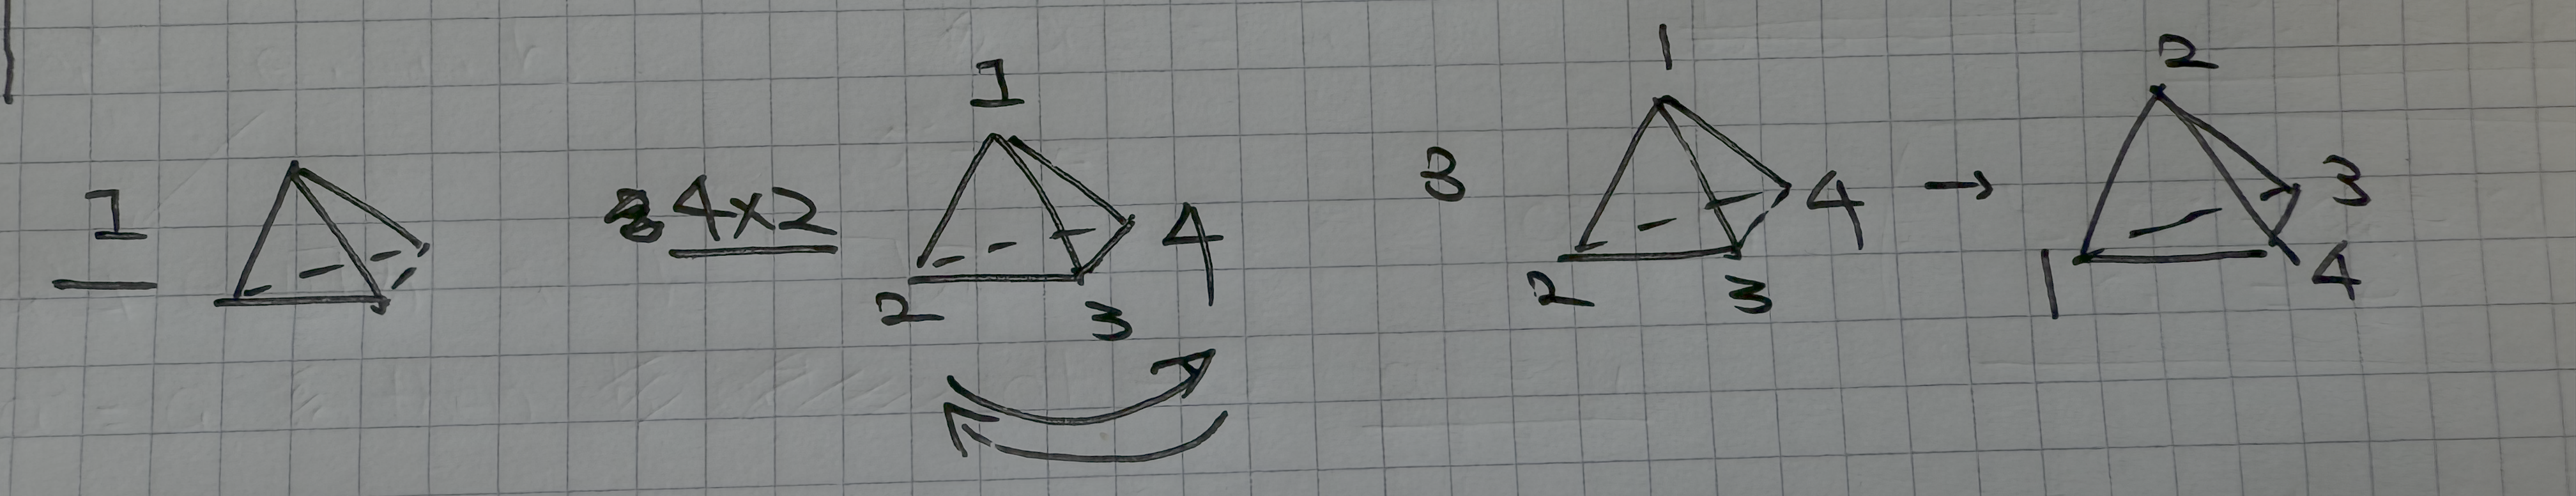
\includegraphics[width=0.75\textwidth]{assets/illustrationtetra.png}
  \caption{Illustration of 3 kinds of moves}
  \label{fig:illustrationtetra}
\end{figure}
We now list out the group elements using the notation of the permutation group (Its obvious that this is a subgroup of $ S_4 $):
\begin{equation}
  \begin{aligned}
    &e\\ 
    &r_1 = (2,3,4),\  r_2 = (1,4,3), \ r_3 = (1,2,4), \ r_4 = (1,3,2)\\ 
    &r_1' = (2,4,3),\  r_2' = (1,3,4),\  r_3' = (1,4,2),\  r_4' = (1,2,3)\\
    &f_{1,2} = (1,2)(3,4),\  f_{1,3} = (1,3)(2,4),\  f_{1,4} = (1,4)(2,3)\\ 
  \end{aligned}
  \label{eq:tetrahedralgroup}
\end{equation}
Consider that the number of conjugacy classes is equal to the number of irreducible representations. And from $ \sum_a n_a  = 12$ we can guess that there are 4 conjugation classes $ 9+1+1+1 = 12 $ or 6 conjugation classes $ 4+4+1+1+1+1 = 12 $. However, by observing the symmetry and doing the exact calculation the 4 conjugation class hypothesis seems to be more resonable. We have: $ e $ as a single conjugation class; $ r_1,r_2,r_3,r_4 $ as a conjugation class; $ r_1',r_2',r_3',r_4' $ as a conjugation class; $ f_{1,2},f_{1,3},f_{1,4} $ as a conjugation class. We deonte the 4 conjugation classes as $ e, r, r', f $. 

we then notice that the $ f $ conjugation class is not just a conjugation class, it is also an invariant subgroup when we add $ e $ in. So we can construct the factor group $ G / H $ where $ H = \{ e, f_{1,2},f_{1,3},f_{1,4} \} $. We figure out that the factor group has only 3 elements $ H, Hs = s, Hs' = s' $ Note that 3 order group is unique so it must be isomorphic to $ \mathbb{Z}_3 $ group. 

So the irreducable representation of $ \mathbb{Z}_3 $ group also forms a representation of the tetrahedral group. There are 2 non-trivial irreducable representations of $ \mathbb{Z}_3 $ group, $ D_1(g) = e^{2/3 \pi i}, D_1'(g) = e^{4/3 \pi i} $. Thus we list out the character table: 

\[
 \begin{array}{c|cccc}
  & e & r & r' & f\\
\hline
    D_0  & 1 & 1 & 1 & 1 \\
    D_1  &  1  & e^{2/3\pi i} & e^{4/3\pi i} &  1 \\
    D_1'  &  1 &  e^{4/3\pi i}& e^{2/3\pi i}& 1 \\
    D_3  & 3 &  &  & \\
\end{array}
\]

Then from the orthogonality of character we can figure out that the last representation is 3 dimensional and its character is $ 3,0,0,-1 $.

it is worth noting that the 4 dim character table is orthogonal vertically (we view evey column as a vector) but not horizontally. This is because the orthogonality of character is only guaranteed when we consider the sum over all group elements, not just the conjugation classes. So we need to multiply the number of elements in each conjugation class when we consider the orthogonality.


